\documentclass[a4paper,11pt]{report}
%FONT size can be changed on the above line
\usepackage[left=2.7cm,right=2.7cm,top=4cm,bottom=3.5cm,bindingoffset=0cm]{geometry}
%%% Headers
\usepackage{fancyhdr}
\renewcommand{\chaptermark}[1]{%
\markboth{#1}{}}  
\pagestyle{fancy}
\fancyhead[LO]{}
\fancyhead[RE]{}
\fancyhead[LE]{\textit{\leftmark}}
\setlength{\headheight}{15pt}

%%%%
\usepackage{tabularx}
\usepackage{amsmath}
\usepackage{amssymb}
\usepackage{ntheorem}
\usepackage{graphicx}
\usepackage{setspace}
\usepackage[outdir=./]{epstopdf}
\usepackage{caption}
\usepackage{subcaption}
\usepackage{array}
\usepackage{paralist} 
\usepackage{datetime}
\usepackage{verbatim}
\usepackage{makeidx}
\usepackage{titling}
\usepackage{titlepic}
\usepackage{enumitem}
\usepackage[toc,page]{appendix}
\usepackage[breaklinks=true]{hyperref}
\usepackage{pdfpages}
\usepackage{mathrsfs}
\usepackage{etaremune}
 \usepackage{bm}
\usepackage{sansmath}
\usepackage{pgfplots}
\usepackage{mdframed}
\usepackage{tikz}
\usepackage{float}
\usepackage{tikz-3dplot}
\usepackage{stmaryrd}
%%Fix line breaks for long citations
\usepackage{breakcites}
\usepackage{siunitx}
\usepackage{tocbibind}
\usepackage{lipsum}
\usepackage{minted}

\renewcommand{\epsilon}{\varepsilon}
\usepackage[style=ieee]{biblatex}

\addbibresource{references.bib}

\mdfdefinestyle{MyFrame}{%
%    linecolor=blue,
        linewidth=1pt,
%    roundcorner=20pt,
%    innertopmargin=\baselineskip,
%    innerbottommargin=\baselineskip,
%   innerrightmargin=20pt,
%    innerleftmargin=20pt,
%    backgroundcolor=gray!50!white
}
\usepackage{svg}
\usepackage{listings}
%New colors defined below
\definecolor{codegreen}{rgb}{0,0.4,0}
\definecolor{codegray}{rgb}{0.5,0.5,0.5}
\definecolor{codepurple}{rgb}{0.58,0,0.82}
\definecolor{backcolour}{rgb}{0.95,0.95,0.92}

\lstdefinestyle{mystyle}{
  backgroundcolor=\color{backcolour}, commentstyle=\color{codegreen},
  keywordstyle=\color{magenta},
  numberstyle=\tiny\color{codegray},
  stringstyle=\color{codepurple},
  basicstyle=\ttfamily\small,
  breakatwhitespace=false,         
  breaklines=true,                 
  captionpos=b,                    
  keepspaces=true,                 
  numbers=left,                    
  numbersep=5pt,                  
  showspaces=false,                
  showstringspaces=false,
  showtabs=false,                  
  tabsize=4
}
\lstset{style=mystyle,upquote=true}

\begin{document}


\begin{titlepage}
    \begin{center}

    \vspace{30pt}
    
\includegraphics[width=0.5\textwidth]{figures/ATULogo.png}\\
    \vspace{50pt}
    
    \fontsize{14}{20} \selectfont
    \setstretch{2.0}{\textbf{\Huge Automated Detection of COVID-19 using Convolutional Neural Networks and Generative Adversarial Networks}} 
    \vspace{20pt}
    
    A thesis submitted \\
    by\\
    \vspace{10pt}
    
    {\huge Ultan Kearns}\\
    \vspace{10pt}
    
     in partial fulfillment of the requirements for the degree of\\ Master of Science in Computing in Big Data Analytics and Artificial Intelligence
    \vspace{20pt}

%        \fontsize{16}{20} \selectfont
    
    
    Supervisor: Dr Paul Greaney
    \vspace{30pt}
    
    
Submitted to Quality and Qualifications Ireland (QQI) \\
Dearbhú Cáilíochta agus Cáilíochtaí Éireann
    \centerline{\monthname \quad \the\year}
\end{center}    
\end{titlepage}

\onehalfspace


\setcounter{page}{1}

%\setcounter{tocdepth}{2}

\addtocontents{toc}{\protect\setcounter{tocdepth}{-1}}
\tableofcontents
\addtocontents{toc}{\protect\setcounter{tocdepth}{2}}

%\listoffigures

\chapter*{Declaration}
\addcontentsline{toc}{chapter}{Declaration}

I hereby certify that this material, which l now submit for assessment on the programme of study leading to the award of Master of Science in Computing in Big Data Analytics and Artificial Intelligence, is entirely my own work and has not been taken from the work of others except and to the extent that such work has been cited and acknowledged within the text of my own work. No portion of the work contained in this thesis has been submitted in support of an application for another degree or qualification to this or any other institution. I understand that it is my responsibility to ensure that I have adhered to LYIT’s rules and regulations. 
\bigskip

I hereby certify that the material on which I have relied on for the purpose of my assessment is not deemed as personal data under the GDPR Regulations. Personal data is any data from living people that can be identified. Any personal data used for the purpose of my assessment has been psuedonymised and the data set and identifiers are not held by LYIT. Alternatively, personal data has been anonymised in line with the Data Protection Commissioners Guidelines on Anonymisation.
\bigskip

I give consent for my work to be held for the purposes of education assistance to future Computing students at LYIT and it will not be shared outside the Department of Computing at LYIT. I understand that my assessment may be shared with any other third party and will be held securely in LYIT in line with the Institute's Records Retention Policy. 

\vspace{20pt}

\hspace{60pt} Signed: \underline{\quad \quad Ultan Kearns\hspace{240pt}} 


\bigskip

\hspace{70pt} Date: \underline{\quad \quad\today\hspace{150pt}} 
\chapter*{Acknowledgements}
\addcontentsline{toc}{chapter}{Acknowledgements}
I would first of all like to thank my supervisor during this project Dr. Paul Greaney, he was a fantastic help throughout the course of writing this thesis and this work could not have been completed without his input and help.
\\[1.5cm]
I would also like to thank the lecturers who taught me so much during my postgraduate course, both Doctors Karla Muñoz-Esqueival and Shagufta Henna provided a fantastic introduction into many areas of Artificial Intelligence and the knowledge they imparted has helped me a lot throughout the course of conducting this research. 
\\[1.5cm]
I would also like to thank Andrew Ng, his deep learning courses provided a great foundation into the realm of deep learning and Artificial Intelligence.
\\[1.5cm]
I would like to thank Francois Chollet whose book ``Deep Learning with Python`` was an indispensible resource and helped me get more familiar with the Keras library as well as the best AI practices and concepts such as transfer learning.
\\[1.5cm]
Finally I would like to thank my parents,and friends for supporting me throughout the course of this masters.

\chapter*{Acronyms}
\addcontentsline{toc}{chapter}{Acronyms}
\begin{table}[h]
    \centering
    \begin{tabular}{|c|c|}
        \hline
         Acronym
         &  Stands For\\
        \hline
        AI & Artificial Intelligence\\
        ANN & Artificial Neural Network\\
        CNN & Convolutional Neural Network\\
        GAN & Generative Adversarial Network\\
        CT & Computed Topography\\
        LSTM & Long short term memory\\
        AUC & Area under curve\\
        DCNN & Deep Convolutional Neural Network\\
        RCNN & Regions with CNN Features\\
        VAE & Varational Auto Encoder\\
        DCGAN & Deep Convolutional Generative Adversarial Network\\
        \hline
    \end{tabular}
    \caption{Acronyms used in this thesis}
    \label{tab:Table of Acronyms}

\end{table}
 


\listoffigures
\listoftables
\begin{abstract}
    This paper aims to analyze the applications of generative adversarial networks or GANs in overcoming issues of data-shortages in relation to developing convolutional neural networks to automate the diagnosis of COVID-19 in patients.  There have been many COVID-19 data-sets compiled but some suffer from lack of data-quality and data shortages\cite{covid19DataQuality}\cite{covid19DataQuality2}.  In this paper I aim to create and train multiple convolutional neural networks or CNNs to analyze X-Rays of patients lungs to automate the detection of COVID-19.  The CNN will be trained with a number of images generated from different GAN architectures to determine which will prove most efficient in automating the detection of COVID-19.  I also aim to use the GANs in conjunction with one and other to try out different combinations to see if feeding images generated by one GAN to other GANs will produce more accurate results when training the model.  In the results section of this Thesis I will compare and contrast the results of the various architectures and determine which proved most effective in it's diagnostic potential.
\end{abstract}

\chapter{Introduction}

\section{Explanation of Generative Adversarial Networks (GANs)}
A generative adversarial network or GAN for short first appeared in a 2014 paper by Ian Goodfellow et al\cite{generativeAdversarialNetworks}.  In this paper Goodfellow et al propose a new way to generate data via an adversarial process.  The GAN essentially works as follows: two models are trained, a generative model $G$ which will generate the synthetic data from the real data and another model $D$ which will be the discriminator, judging if the data was created by the model or if it came from the dataset.  The goal of this training is to ensure data generated from $G$ is realistic enough to make the discriminator $D$ believe that the generated content came from the training set, this is achieved by training the model for a number of epochs and adjusting the models weights to improve the quality of the generated image.  It  is in this way that we can create realistic "fake" data from the generative model.
\\
There are a number of GAN architectures which are useful in different scenarios, such as CycleGans\cite{cycleGan} which are useful for translating images from a source domain $X \rightarrow Y$ in which $Y$ is the target domain, StyleGan, which was created by NVIDIA which allows more control over the generative process\cite{styleGan} and PixelRNN, which can recreate images when given a fraction of the original and can generate new images based on probability\cite{pixelRnn}. 
\\
This dissertation examines a number of different generative adversarial network architectures and their ability to produce meaningful data when trained on the datasets which will be mentioned in a later section.
\vspace{0.5mm}
\begin{figure}[H]
    \centering
    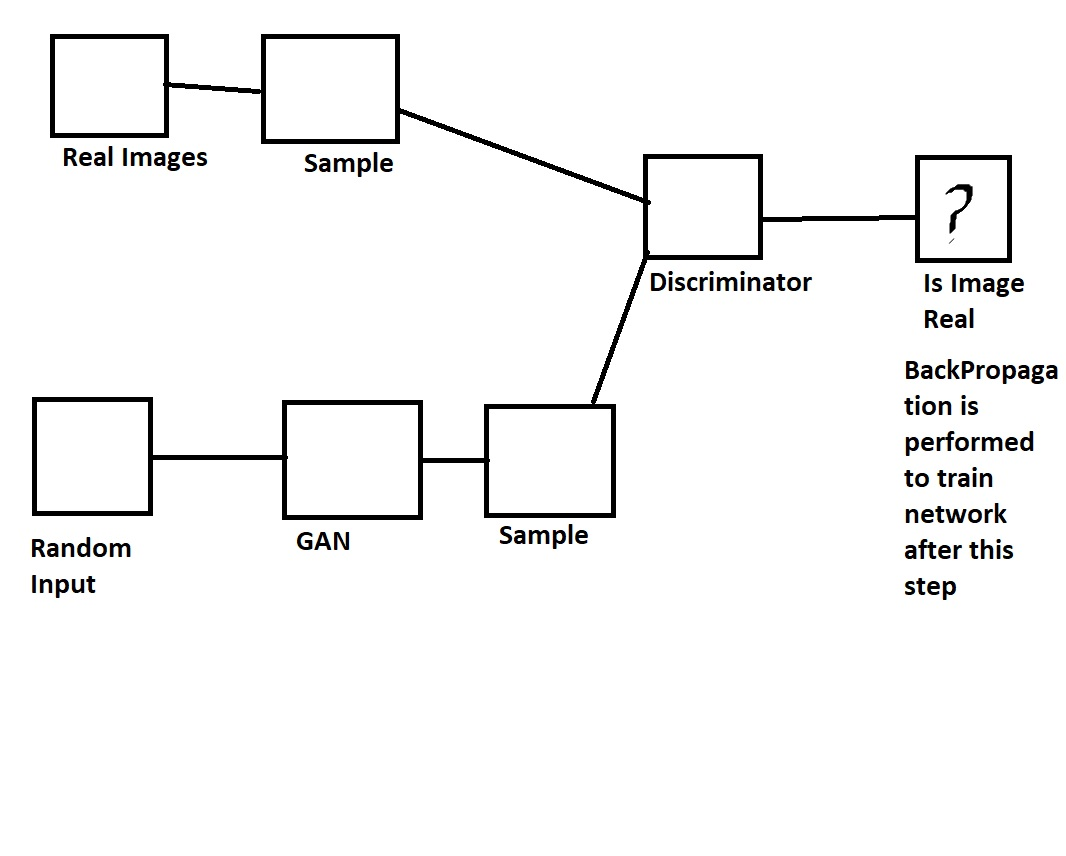
\includegraphics[width=1\textwidth,height=10cm]{Images/GAN Basic.jpg}\\
    \caption{Basic Example of Generative Adversarial Network}
    \label{fig:Example GAN Diagram}
\end{figure}
\vspace{0.5mm}
As we can see from the image above \ref{fig:Example GAN Diagram}, we start the process by taking a sample of real images from the training data, then passing it to the discriminator. We also take a sample from the GAN created images and pass that to the discriminator which will then determine if the images are real are fake.  After the discriminator guesses if the image generated is good enough to be considered real in terms of quality then backpropagation is performed to train the model so that it can differentiate better between samples that came from the training set and those which came from the generator $G$.
\section{Explanation of Artificial Neural Networks (ANNs)}
Artificial Neural Networks, or ANNs for short, comprise of a network of neurons or nodes(both terms can be used interchangeably) which are used for training a model to perform a certain task.  They are made up of an input layer, $N$ hidden layers, and finally an output layer.  Each layer has its own activation function and will adjust its weights and biases to determine the final output of the model.\cite{introToCnn} These networks are  heavily inspired by biological processes which occur in the brain.
\\
Artificial neural networks are a general-purpose model used to solve a number of common problems.
\vspace{0.5mm}
\begin{figure}[H]
    \centering
    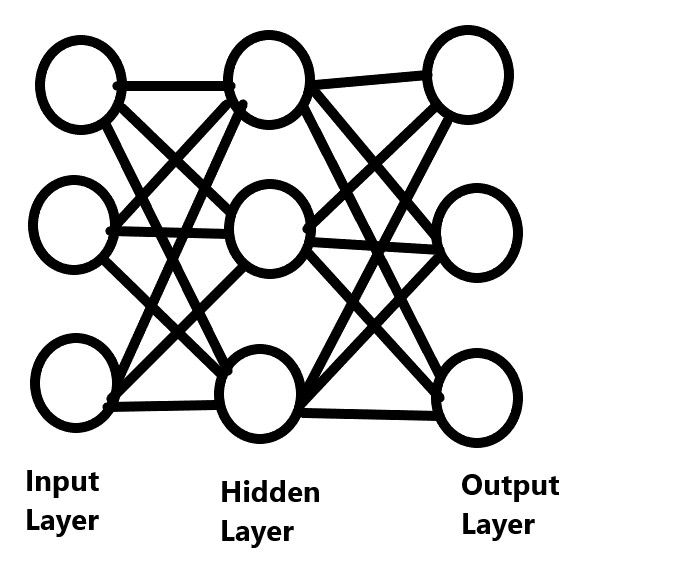
\includegraphics[width=0.5\textwidth]{Images/ANN Basic.jpg}\\
    \caption{Diagram of a Basic Artificial Neural Network with 1 input layer, 1 output layer, and 1 hidden layer}
    \label{fig:Example ANN Diagram}
\end{figure}
\vspace{0.5mm}

A basic example of an artificial neural network is shown in Figure \ref{fig:Example ANN Diagram}. As shown in the figure, the network has an input layer, a hidden layer, and an output layer.  Generally when creating these networks we determine the number of neurons in both the input and the output layers based on the number of classes we are trying to predict.  The above network could be used to predict if an image is of a cat, a dog, or a fish for example.  There can multiple hidden layers in an ANN and the number of neurons in each layer can be adjusted.  In reality, artificial neural networks will typically be far bigger than the example given above in terms of neurons and hidden layers but for illustrative purposes, the above diagram will suffice.  Each neuron will also have its own weight, bias, and an activation function which will determine whether a neuron fires or not. There are many common activation functions such as swish, ReLU (Rectified Linear Units), sigmoid, and tanh the use of which depends on a number of factors.
\section{What is A Convolutional Neural Network? (CNN)}
A convolutional neural network, or CNN for short, is a type of neural network which is primarily used for tasks involving image and pattern recognition\cite{introToCnn}. The structure is similar to an ANN in which we have an input layer, $N$ hidden layers, and finally an output layer.  As with the Artificial Neural Network each of these layers will have an activation function and its own weights and biases to determine the final output for a given input. The model will take an image as input, the image is made up of vectors (RGB) or a similar format and from that image the model will determine certain patterns. For example, the output might be a classification of whether or not COVID-19 is present. This application will be discussed in more detail later in the dissertation. 
\\
There are a few ways in which CNNs differ from ANNs, in that they are comprised of three types of layers which are the convolutional layers, pooling layers, and fully connected layers\cite{introToCnn}.  The convolutional layer is responsible for extracting features from an image and generating a $2D$ activation map, the pooling layer will reduce the parameters of a given input by means of downsampling, and finally the fully connected layers will then determine and classify the output for a given input.  The convolutional layer's parameters utilize learnable kernels (a kernel acts as a filter used to extract features from images), and this layer also produces a $2D$ activation map which will be used to determine if a neuron fires or not for a given input.  We can adjust hyper parameters in the convolutional layer to greatly reduce the complexity of the model through optimization, which can be achieved by adjusting the following hyper parameters: depth, stride and zero padding.
\\
Depth is related to the output volume produced by the convolutional layers in the model which can be manually set by adjusting the number of neurons in each layer.  Reducing the depth of the model can greatly decrease the training time but at the expense of performance.
\\
Stride is related to the spatial dimensionality of the input which will determine the receptive field (this is an area where each neuron in the network is connected to a small region of the input - this area of the network is called the receptive field\cite{introToCnn}), if the stride is set to a low integer we will produce extremely large activations, and if it is set too high the network won't produce enough activations.  The stride can also be interpreted as sliding a window across the image / video, where only a section of the image or video is input into the network at a time.
\\
Finally, zero-padding will pad the border of the images ingested by the model with 0s, reducing their dimensionality. Padding can prove to be useful in increasing the accuracy of the model as it can possibly eliminate areas of the image which are not useful for the model and can also improve training time times in some use cases\cite{zeroPaddingTrainingTime}.
\\
Through the adjustment of the hyperparameters mentioned above, and through the utilization of different activation functions, the accuracy of the convolutional neural network can be improved through a process of trial and error.
\section{Supervised Learning}
Supervised learning is a methodology of machine-learning involving the use of labeled data to train the model\cite{supervisedVsUnsupervised}. The data is typically labeled manually by a data scientist, which can be a long and laborious process depending on a number of factors (size of the data, number of classes, etc.), but offers many benefits when it comes to training models.  Supervised learning performs extremely well at tasks involving classification (classifying data into a given category), and regression (understanding the relationships between independent and dependent variables). 
\section{Unsupervised Learning}
Unsupervised learning is a methodology of machine-learning which involves using unlabelled data to train machine learning models\cite{supervisedVsUnsupervised}.  This type of machine learning requires no human intervention since the data is unlabelled and the model will detect relationships between data based on the raw data fed in to the model.  This type of machine learning is used for tasks such as: clustering (grouping data together based on shared characteristics or features), association (finding relationships between features), and dimensionality reduction (reducing the number of features in a given dataset without compromising the integrity of said data).  The key differences between supervised and unsupervised learning are: labeled versus unlabeled datasets, and finding relationships in data (unsupervised) or trying to predict and classify data (supervised).
\section{Tensorflow}
Tensorflow is an open-source library which allows developers to access a number of functions to make machine learning easier and allows developers to build models more quickly\cite{tensorflow}.  Tensorflow provides numerous modules and classes which form the foundation for building both the generative adversarial network and the convolutional neural network. There have been numerous case studies proving the efficacy of Tensorflow in solving many AI / ML problems and the library is used by research teams in organisations such as Google, Airbnb, ARM, Coca-Cola, Intel, and many more\cite{tensorflowCaseStudies}.  
\\
Given the reputation and widespread use of Tensorflow, and the vast amount of documentation around the framework, it seems  an ideal library for the implementation of GANs and CNNs for this study.
\section{Keras}
Keras is a deep-learning framework for Python developed by Francois Chollet which provides a number of helpful functions and methods for creating AI models\cite{keras}. Keras is built on top of Tensorflow and simplifies data loading, pre-processing and the overall building of the model.  Keras is commonly used by data-scientists and researchers due to the powerful methods it offers and the time it saves.  The additional classes and modules Keras provides on top of Tensorflow will help to reduce the time taken to build and develop of building both the convolutional neural network and the generative adversarial network.  
\\
Like Tensorflow, Keras has been used by a number of companies and is well recognised in the Artificial Intelligence community.  The framework has a range of uses and has proven beneficial when developing AI models in a number of areas and fields\cite{kerasExamples}.
\section{Background of Problem \& Aims of This Paper}
COVID-19 is a highly transmissible virus which has caused a worldwide pandemic and has claimed many lives. There have been 616,951,418 cases worldwide and 6,530,281 deaths as of the 4th of October 2022\cite{covid19StatsWorldwide}.  During the pandemic, Ireland alone was subject to a total of 1.6 million confirmed cases and nearly 8,000 deaths\cite{covid19StatsIreland}.  This has led many researchers to pursue the goal of automating the detection of COVID-19 to partially relieve the immense pressure put on medical staff throughout the pandemic. 
\vspace{0.5mm}
\begin{figure}[H]
    \centering
    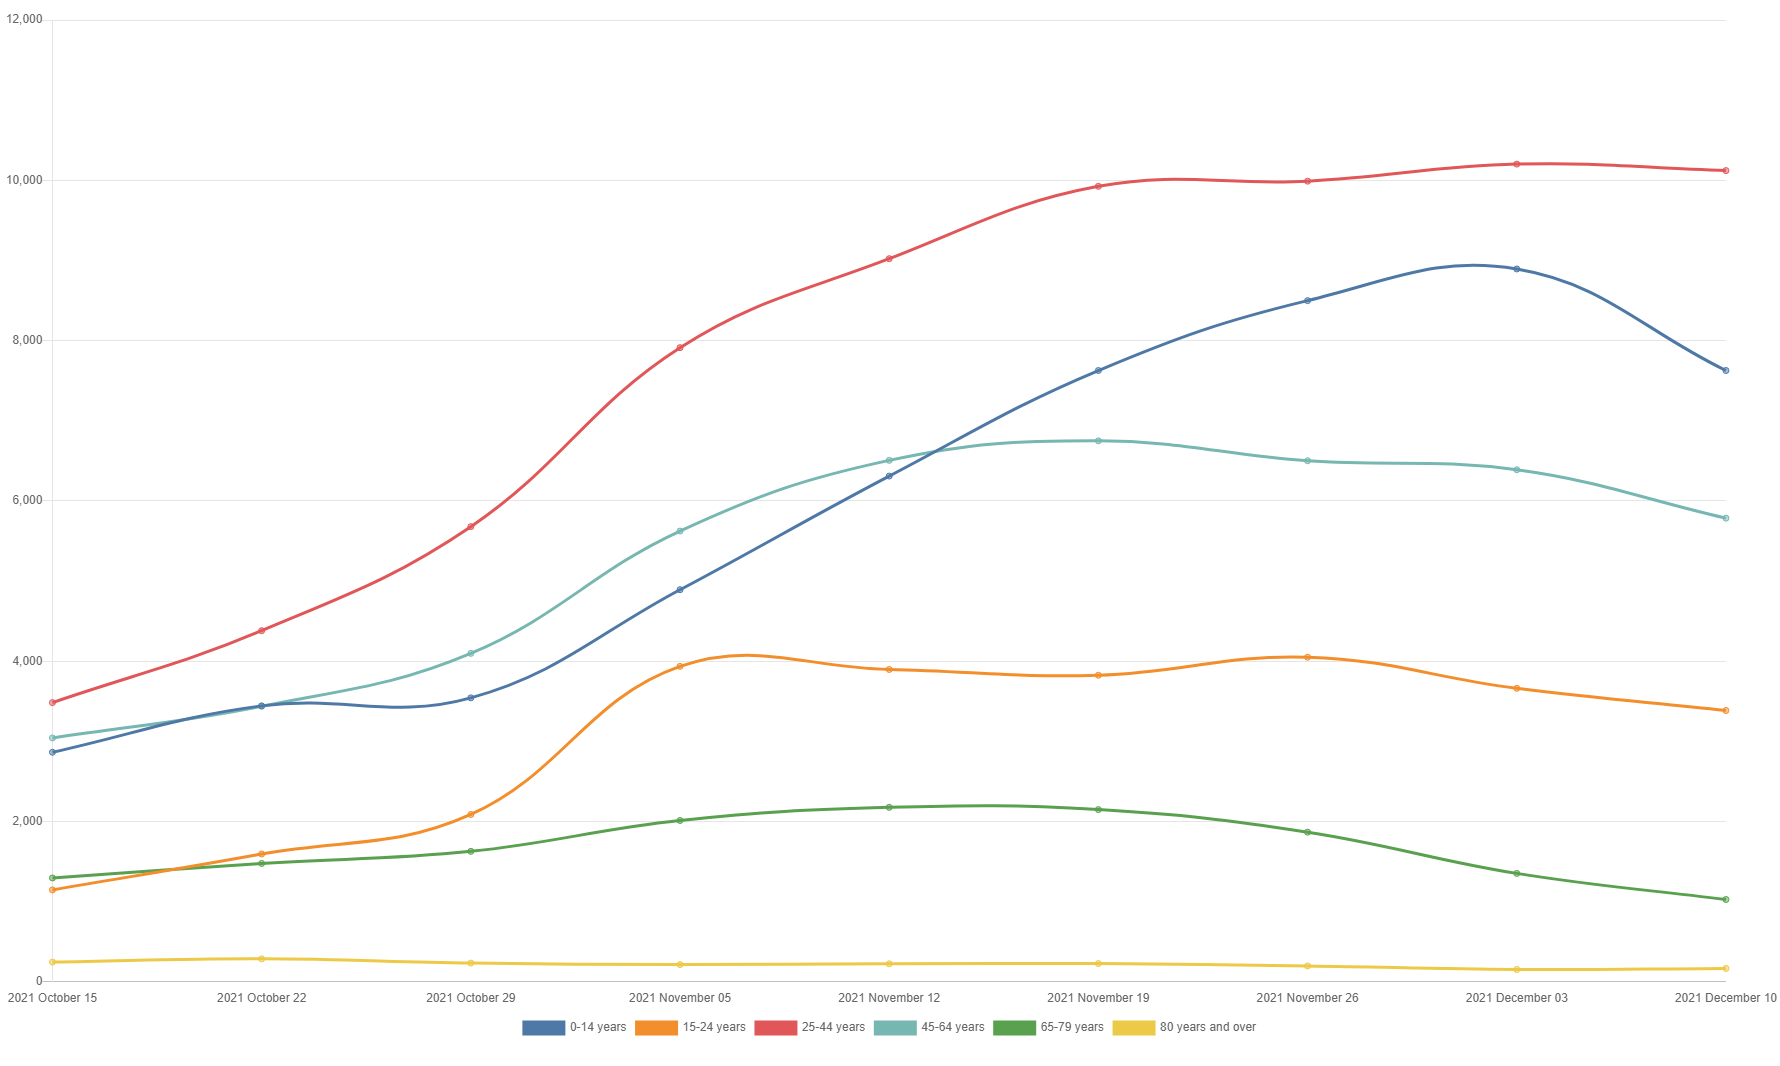
\includegraphics[width=1\textwidth,keepaspectratio]{Images/COVID19IrelandFigures.png}\\
    \caption{Graph of COVID-19 Statistics by age-range Ireland from October 2021 - December 2021 Courtesy of CSO\cite{csoCovid19Stats}}
    \label{fig:COVID-19 Ireland Statistics}
\end{figure}
\begin{figure}[H]
    \centering
    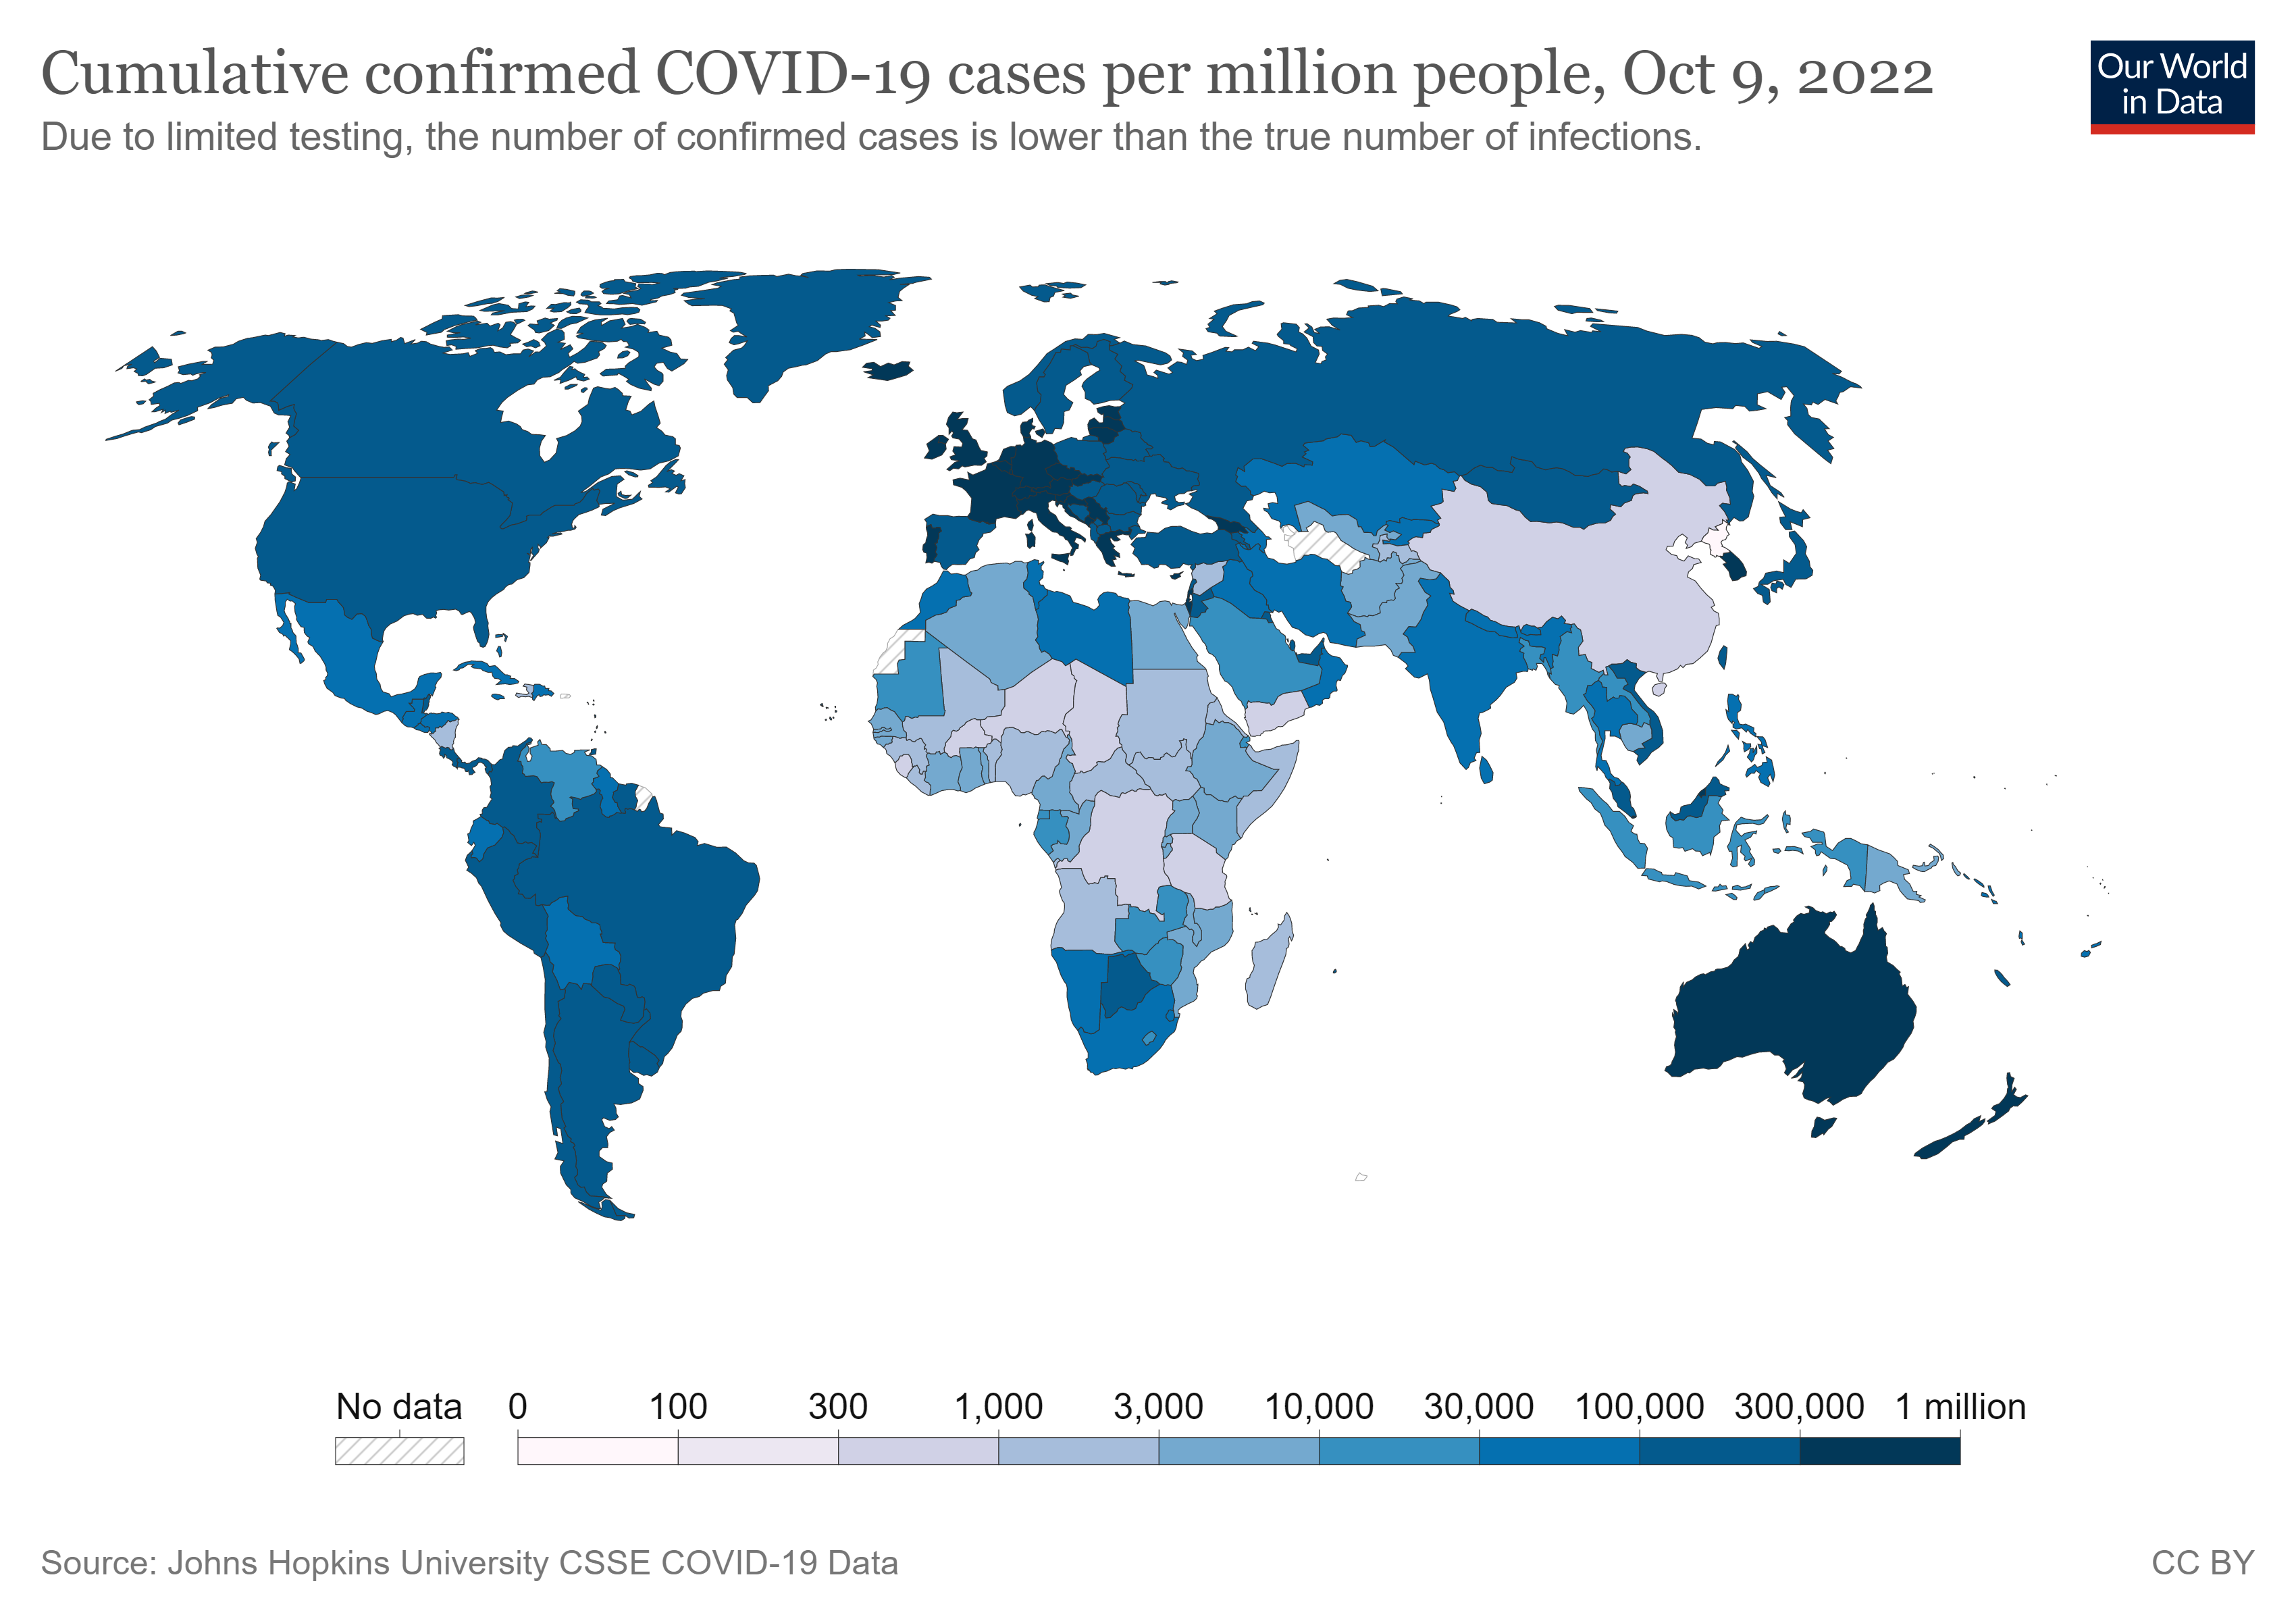
\includegraphics[width=1\textwidth,keepaspectratio]{Images/coronavirusWorldWide.png}\\
    \caption{Cumulative cases of the COVID-19 virus worldwide courtesy of Our World in Data\cite{cumulativeCovid19Cases}}
    \label{fig:COVID-19 Worldwide Statistics}
\end{figure}
\vspace{0.5mm}
The main objective of this research is to develop a robust model which can accurately analyze X-rays of patients and determine from said X-rays if the patient is afflicted with COVID-19.  This will be achieved by utilizing a number of different GAN architectures which will create realistic ''fake data'' which will then be used to train a number of models. From this training we plan to compare and contrast the results when generating data with different architectures to determine the best configuration for data generation to train the CNN model.  There has been some success in utilizing convolutional neural networks to automate the detection of the virus\cite{cnnCOVID19DetectionAhmed}\cite{cnnCOVID19DetectionLopez}.  Through the use of synthetic data generated by utilizing a variety of GAN architectures, it is our hope that such convolutional models will be improved upon and made more accurate.
\\
We plan on utilizing existing data sets which are listed in the next section when training the Generative Adversarial Models, through trial and error we plan on determining the best architecture of GANs to use for training the model for this use-case.
% Include stats and explain COVID 19 virus
\section{Datasets}
Before beginning the training of the model it is important to explore and understand each of the datasets.  There are a total of three datasets which will be used in the course of this research, we will explain more about these datasets below.
\subsection{COVID-19 Chest X-ray}
The COVID-19 Chest X-ray data set is a data set which is comprised of labeled X-ray Images taken from a number of patients. This dataset contains 357 X-ray images of COVID positive patients, and Chest X-rays of those afflicted with another disease (MERS, SARS, and ARDS).  This dataset also includes a metadata file listing the diagnosis of the patient along with a number of other features\cite{xrayDataset}. In total this dataset contains 11 classes, the images do not have a consistent resolution which may cause issues as resizing each image may lead to a loss in image quality.  The loss in quality will cause problems when evaluating the model's accuracy.
\\
\subsection{COVID-19 Radiography Database}
The COVID-19 Radiography Database is made up of 3,616 images of chest X-rays taken from COVID positive patients, 10,192 Images of lung X-rays taken from healthy patients, and 1,345 X-ray images of viral pneumonia positive patients. All images in this dataset are PNG (Portable Network Graphic) images and are at a resolution of height 299 pixels and width 299 pixels eliminating the need for preprocessing of the images, the dataset also includes metadata for each of the images in this dataset showing a number of features with the diagnosis of the patient as well. The data in this dataset was gathered by a team of researchers from Qatar University, Doha, Qatar, and the University of Dhaka, Bangladesh along with their collaborators from Pakistan and Malaysia\cite{radiography}.
\\
\subsection{COVID-19 Pneumonia Normal Chest X-ray PA Dataset}
The COVID-19 Pneumonia Normal Chest X-ray PA dataset is comprised of a train set containing 74 Normal X-ray Images taken from healthy Patients and  afflicted with Pneumonia and a test set containing a Normal set containing 20 chest X-rays taken from healthy patients and a Pneumonia set containing 20 images.  The images in this dataset are unlabelled and no metadata is offered, however, the images are segregated into separate files listing the diagnosis\cite{covidDataset}.
\\
\subsection{Extensive COVID-19 X-ray and CT Chest Images Dataset}
This dataset was added fairly late in the project due to data limitations in both the COVID-19 Chest X-ray and the COVID-19 Pneumonia Normal Chest X-ray PA Dataset.  This dataset is comprised of 17099 X-ray and CT images which were generated with various augmentation techniques.  Some of the images in this dataset come from the previously mentioned datasets namely the COVID-19 Pneumonia Normal Chest X-ray PA Dataset and the COVID-19 Chest X-ray.  Given the large number of images in this dataset it may prove useful when training GANs to reproduce images as some of the other datasets have proven to lack the data needed to reasonably train a GAN to reproduce the X-rays.
\\
The dataset is broken up into two folders containing X-rays and CT Scans respectively. Both folders contain images which are categorized into two further subfolders 
one containing COVID Positive X-ray and CT-Scans and the other containing COVID negative X-ray and CT scans\cite{extendedCOVIDds}.
\\
\subsection{Use of datasets in This Project}
we plan to use each of these datasets to train and test the model and use data augmentation to increase the train and test sets by utilizing Generalized Adversarial Networks.  When using these datasets in conjunction it is my hope that the GAN will have enough data to be effective when generating new sample images to train the final model.

\section{Structure of This Thesis}
This thesis is broken into 5 chapters in total, this section will include the headings of the chapters and a brief summary of each chapter below:

\subsection{Chapter 1 - Introduction} 
This chapter will offer the reader of this thesis a brief introduction to a number of core concepts which will be necessary to understand before diving deeper into this thesis.  It is important that the reader has a basic understanding of generative adversarial networks, convolutional neural networks, artificial neural networks, supervised \& unsupervised learning, and the overall question that this research proposes before discussing the implementation or discussing pertinent literature in this field. 
\\
In this section we will frame the research question, explain what a generative adversarial network is, its function, and how it works,  We will also explain artificial neural networks and convolutional neural networks, and we will discuss the basic methodologies relating to the implementation of this project.  We will also discuss the libraries used to implement the practical artifact, datasets used to train the model and give the reader of this thesis a clear understanding of the key aims of this research.
\subsection{Chapter 2 - Literature Review} 
In this section we will review pertinent literature related to the problem domain and discuss the ideas and concepts presented in these papers. We will also review the results from the research conducted in these papers and use them as a metric to gauge the performance of my own model.  The papers will also be compared and contrasted and we will discuss the findings and how useful these papers were when conducting my own research.  It is very important to understand the problem domain before beginning the implementation of this project to ensure that we are not "reinventing the wheel".  This section will also provide the reader of this thesis with the most up-to-date progress made within the problem domain.
\subsection{Chapter 3 - Implementation}
In this section we will discuss the architecture of the convolutional model, the various architectures of generative adversarial networks implemented, how the models were trained and the overall design of the code implemented, and the rationale behind certain design choices. we will also show the results from training the models and discuss how through trial and error we were able to improve the various models and will include code samples so that the models can be reviewed by the reader or re-implemented by them.
\subsection{Chapter 4 - Results}
In this section, we will review the results achieved from training the best models and suggest how they may possibly be improved.  we will be showing lots of graphs/tables in this section to gauge each model's test/dev set errors and we will also be comparing and contrasting the effects of the different GAN architectures implemented as well as discussing the results of the convolutional model.
\subsection{Chapter 5 - Further Research and Conclusions}
In this section, we will discuss further research that may need to be done by any researchers who would like to build upon this research.  we will also review where the models could be improved and what we'd do differently if we were to conduct this research again. we will also discuss common issues we faced during the implementation of this project and how we overcame them. This section will be a summary of all the research conducted, the code, and my experience overall throughout the writing of this thesis.  
\\
This will be the final section of the paper and will tie the entire thesis together.  

 

\include{chapter 2 literature review}
\chapter{Implementation}
\section{Introduction}
Initially, when starting the development of this model, we looked at various tools and options to implement the model in code.  We settled on using Jupyter Notebooks along with a number of libraries to help make the development of this model easier and faster.  The useful thing about Jupyter Notebooks is that they can be opened in a browser and all the code can be run from a single page.  We will detail the development of this model both in this thesis and include notes in the notebook itself to explain my rationale behind implementing the model in a certain way.  During the initial phase of implementation, I used both the Keras documentation \cite{keras} and Tensorflow documentation \cite{tensorflow} as references to ensure that the model's development was following standard practices and to ensure that the model was optimized to allow training in a timely manner. 
\\
Due to the limited support for AMD graphics cards(currently I use a 6700XT which does not have RoCM support\cite{amdLimitations}) in a variety of popular AI frameworks/libraries at the time of my writing this thesis, we decided it was best to use Google Colab Pro when training both the CNNs and the GANs this may offer some limitations in terms of memory and computational power.  Google Colab Pro, however, does offer a lot of advantages when it comes to quickly setting up an environment in which to train these models, it is for this reason that I have chosen to use it for training the models.
\\
For the purpose of reproducible results, we included the following lines of code np.random.seed(9) and set the random seed of Keras to 10 so that other researchers can reproduce the results and build upon this study.  All the datasets are loaded and split using a seed of 1337 also so that the train/test split is the exact same every time.
\section{CNN Baseline Model Design and Comparison}
When starting the implementation phase, we decided to use the following resource to develop baseline CNN models\cite{imageClassificationKeras}.  We plan on modifying this resource to achieve a relatively high training/validation accuracy when training on the original dataset.  We plan on using these models to get a metric with which we can compare models generated on the original dataset to the models which are generated on the synthetic dataset.  It is in this way we can accurately compare the effects of the synthetic dataset on the accuracy of the implemented models.
\\
After this initial comparison is done with the models trained on the original dataset versus the models trained on the synthetic dataset.  We then plan on focusing on which architectures would work best when developing the CNN and how the models trained on the synthetic dataset can be improved.
\\
To start I decided to use the following settings when developing a CNN to be used when training on the x-ray COVID-19 dataset.  This dataset is made up of images that are labeled either 1 or 0 with 1 being COVID-positive and 0 being COVID-negative.  I have included the architecture of the layers of the model in the table below\ref{tab:First CNN baseline model architecture for X-ray COVID-19 dataset}
\begin{table}[H]
    \centering
    \resizebox{\textwidth}{!}{
    \begin{tabular}{|c|c|c|c|c|c|c|}
    \hline
        Layer Number 
        & Layer Type
        & Layer Size 
        & Kernel Size
        & Strides
        & Padding
        & Activation\\
        \hline
        1 & Conv2D Layer & 16 & (3,3) & 2 & Same & Swish\\
        2 & SeparableConv2D Layer & 32 & (3,3) & 2 & Same & Swish \\
        3  & SeparableConv2D Layer & 64 & (3,3) & 2 & Same & Swish \\
        4  & MaxPooling2D & 2 & 2 & None & Same & None \\
        5 & Residual & 128 & (3,3) & 2 & Same & Swish \\
        6 & SeparableConv2D & 256 & (3,3) & None & Same & Swish \\
        7 & GlobalAveragePooling2D & 1 & None & None & None & Sigmoid \\
        \hline
    \end{tabular}
    }
    \caption{First CNN baseline model architecture for X-ray COVID-19 dataset}
    \label{tab:First CNN baseline model architecture for X-ray COVID-19 dataset}
\end{table}
For the padding the keyword ''same'' means that the input is padded with 0s evenly, both up and down and left and right of the image. The input was also scaled to normalize the data using the following line of code ''1.0 / 255)(inputs)''  After each layer batch normalization was performed excluding the residual, max pooling, and global average pooling 2D layers.  The use of the activation function ``swish`` was chosen due to studies showing it's performance matched or outperformed ReLU for certain tasks\cite{swishAndRelu}. Swish differs slightly in comparison to ReLU in that there isn't a sharp rise as the weight approaches 0. 
 \begin{figure}[H]
    \centering
    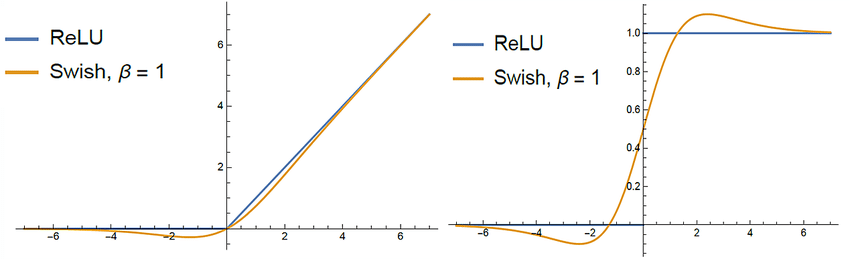
\includegraphics[width=1\textwidth,height=15cm,keepaspectratio]{Images/Swish ReLU activations.PNG}\\
    \caption{Figure of Swish and ReLU activation functions(Image courtesy of Madhura Ingalhalikar)\cite{swishReluDiagram}}
    \label{fig:Figure of Swish and ReLU activation functions}
\end{figure}
The model uses a dropout of 0, given the small size of the dataset I didn't want to drop neurons from the network.  The model was trained using a 70/30 training-validation split as I found this worked the best when training and testing the model. I also used the following settings when using model.compile() 
\begin{table}[H]
    \centering
    \resizebox{\textwidth}{!}{
    \begin{tabular}{|c|c|c|c|c|c|}
    \hline
         Optimizer
         & Loss Function 
         & Metric
         & Batch Size
         & Steps Per Epoch
         & Number of Epochs\\
         \hline
         Adam with a learning rate of $1e-3$ & Binary CrossEntropy & Accuracy & 16 & 1 & 9\\
         \hline
    \end{tabular}
    }
    \caption{First CNN baseline model hyperparameters for X-ray COVID-19 dataset}
    \label{tab:First CNN baseline model hyperparameters for X-ray COVID-19 dataset}
\end{table}
The model was trained for a total of 9 epochs with 1 step per epoch (again due to the limitations in the size of the dataset) and achieved the following results.

\begin{table}[H]
    \centering
    \begin{tabular}{|c|c|c|c|}
    \hline
         Training Loss
         & Training Accuracy 
         & Validation Loss
         & Validation Accuracy\\
         \hline
         0.5495  & 1.0000 & 0.6755 & 0.8393\\
         \hline
    \end{tabular}
    \caption{First CNN baseline model results for X-ray COVID-19 dataset}
    \label{tab:First CNN baseline model results for X-ray COVID-19 dataset}
\end{table}
 \begin{figure}[H]
    \centering
    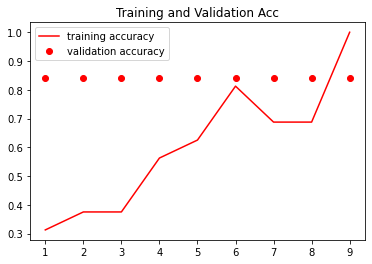
\includegraphics[width=1\textwidth,height=5cm,keepaspectratio]{Images/FirstCNNBaselineTrainAndValAcc.PNG}\\
    \caption{Figure of Train and Validation Accuracy of First CNN Baseline Model}
    \label{fig:First CNN Baseline Train and Validation Accuracy}
\end{figure}
 \begin{figure}[H]
    \centering
    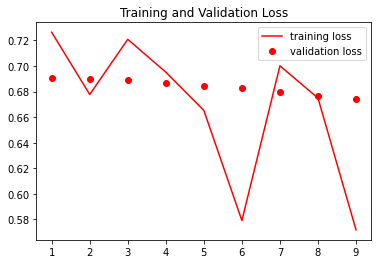
\includegraphics[width=1\textwidth,height=5cm,keepaspectratio]{Images/FirstCNNBaselineTrainAndValLoss.PNG}\\
    \caption{Figure of Train and Validation Loss of First CNN Baseline Model}
    \label{fig:First CNN Baseline Train and Validation Loss}
\end{figure}
As is shown from the results above\ref{tab:First CNN baseline model results for X-ray COVID-19 dataset} the model appears to overfit the training data which is to be expected given the small size of the dataset.  We can also see that the model has a reasonably high accuracy on the validation set but both the training set and the validation set have a high loss which is also caused by the small size of the dataset.
\\
After achieving relatively good performance on the X-ray COVID-19 dataset we then moved on to designing the model with the radiography dataset. This dataset is much larger than the original dataset, the radiography dataset contains a total of 30,306 image files broken into three classes.  In comparison, the X-ray COVID-19 dataset only contains 188 images belonging to two classes.  When designing this Convolutional network more thought had to be given to the split and which activation function to use for output, given that there are multiple classes.  When designing the CNN we decided to implement a much larger neural network given the amount of data available.  We tried using the initial network which was used for the X-ray COVID-19 dataset but the results were poor, increasing the size of the network led to better results.  When training the model I also found that a train/test split of 0.02 worked best using 98\% of the data to train and 2\% to test.
\begin{table}[H]
    \centering
    \resizebox{\textwidth}{!}{
    \begin{tabular}{|c|c|c|c|c|c|c|}
    \hline
        Layer Number 
        & Layer Type
        & Layer Size 
        & Kernel Size
        & Strides
        & Padding
        & Activation\\
        \hline
        1 & Conv2D Layer & 64 & (3,3) & 2 & Same & ReLU\\
        2 & SeparableConv2D Layer & 128 & (3,3) & 2 & Same & ReLU \\
        3  & SeparableConv2D Layer & 256 & (3,3) & 2 & Same & ReLU \\
        4 & SeparableConv2D Layer & 512 & (3,3) & 2 & Same & ReLU \\
        5 & SeparableConv2D Layer & 728 & (3,3) & 2 & Same & ReLU \\
        4  & MaxPooling2D & 3 & 2 & None & Same & None \\
        5 & Residual & 728 & (3,3) & 2 & Same & ReLU \\
        6 & SeparableConv2D & 1024 & (3,3) & None & Same & ReLU \\
        7 & GlobalAveragePooling2D & 3 & None & None & None & Softmax \\
        \hline
    \end{tabular}
    }
    \caption{Second CNN baseline model architecture for COVID Radiography Dataset}
    \label{tab:Second CNN baseline model architecture for COVID Radiography Dataset}
\end{table}


    \begin{table}[H]
    \centering
    \resizebox{\textwidth}{!}{
    \begin{tabular}{|c|c|c|c|c|c|}
    \hline
         Optimizer
         & Loss Function 
         & Metric
         & Batch Size
         & Steps Per Epoch
         & Number of Epochs\\
         \hline
         Adam with a learning rate of $1e-3$ & sparse categorical crossentropy & Accuracy & 32 & 18 & 50\\
         \hline
    \end{tabular}
    }
    \caption{Second CNN baseline model hyperparameters for COVID Radiography Dataset }
    \label{tab:Second CNN baseline model hyperparameters for COVID Radiography Dataset}
\end{table}
In this model we achieved a higher accuracy when using ReLU as opposed to swift the final results of the model are as follows:
\begin{table}[H]
    \centering
    \begin{tabular}{|c|c|c|c|}
    \hline
         Training Loss
         & Training Accuracy 
         & Validation Loss
         & Validation Accuracy\\
         \hline
         0.5146  & 0.7934 & 0.5743  & 0.7508\\
         \hline
    \end{tabular}
    \caption{Second CNN baseline results for COVID Radiography Dataset}
    \label{tab:Second CNN baseline results for COVID Radiography Dataset}
\end{table}
 \begin{figure}[H]
    \centering
    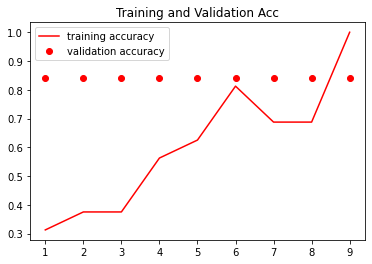
\includegraphics[width=1\textwidth,height=5cm,keepaspectratio]{Images/SecondCNNBaselineTrainAndValAcc.PNG}\\
    \caption{Figure of Train and Validation Accuracy of Second CNN Baseline Model}
    \label{fig:Second CNN Baseline Train and Validation Accuracy}
\end{figure}
 \begin{figure}[H]
    \centering
    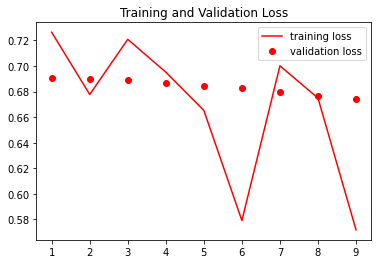
\includegraphics[width=1\textwidth,height=5cm,keepaspectratio]{Images/SecondCNNBaselineTrainAndValLoss.PNG}\\
    \caption{Figure of Train and Validation Loss of Second CNN Baseline Model}
    \label{fig:Second CNN Baseline Train and Validation Loss}
\end{figure}
As shown in the table\ref{tab:Second CNN baseline results for COVID Radiography Dataset} above we can see that the model has worse results when compared with the first baseline model.  The reason for this is due to a number of factors, one being the size of the dataset.  Given that this is a much larger dataset the model will have a more difficult time when classifying the images as there are now far more in the validation set when compared to the first model, there are 606 images for validation in this model as opposed to the 56 images in the first model.
\\
The third and final baseline CNN model was trained using the COVID-19 chest X-ray dataset. This dataset didn't have a standardised resolution for images so the images had to be resized which could possibly lead to lack of data quality and consistency when resized.  When training the model there was a high degree of loss which is to be expected given the data but this may be mitigated when generating images using a GAN which will be in a standardized resolution.  The model was trained with a train / test split of 80\% for the training set and 20\% for the test set.  The architecture of this model is as follows:
\begin{table}[H]
    \centering
    \resizebox{\textwidth}{!}{
    \begin{tabular}{|c|c|c|c|c|c|c|}
    \hline
        Layer Number 
        & Layer Type
        & Layer Size 
        & Kernel Size
        & Strides
        & Padding
        & Activation\\
        \hline
        1 & Conv2D Layer & 32 & (3,3) & 2 & Same & Swish\\
        2 & SeparableConv2D Layer & 64 & (3,3) & 2 & Same & Swish \\
        3  & MaxPooling2D & 11 & 2 & None & Same & None \\
        4 & Residual & 64 & (3,3) & 2 & Same & Swish \\
        5 & SeparableConv2D & 128 & (3,3) & None & Same & Swish \\
        6 & GlobalAveragePooling2D & 11 & None & None & None & Softmax \\
        \hline
    \end{tabular}
    }
    \caption{Third CNN baseline model architecture for COVID-19 Chest X-ray Dataset}
    \label{tab:Third CNN baseline model architecture for COVID-19 Chest X-ray Dataset}
\end{table}

    \begin{table}[H]
    \centering
    \resizebox{\textwidth}{!}{
    \begin{tabular}{|c|c|c|c|c|c|}
    \hline
         Optimizer
         & Loss Function 
         & Metric
         & Batch Size
         & Steps Per Epoch
         & Number of Epochs\\
         \hline
         Adam with a learning rate of $1e-3$ & categorical crossentropy & Accuracy & 10 & 1 & 10\\
         \hline
    \end{tabular}
    }
    \caption{Third CNN baseline model hyperparameters for COVID-19 Chest X-ray Dataset }
    \label{tab:Third CNN baseline model hyperparameters for COVID-19 Chest X-ray Dataset}
\end{table}
Due to the small size of the dataset the batch size was set to a low number. The steps per epoch and number of epochs were also relatively low when compared with the other datasets due to the limited amount of data present.  The model's performance is shown in the table below:
\begin{table}[H]
    \centering
    \begin{tabular}{|c|c|c|c|}
    \hline
         Training Loss
         & Training Accuracy 
         & Validation Loss
         & Validation Accuracy\\
         \hline
         1.6043  & 0.8125 & 2.2768 & 0.6714\\
         \hline
    \end{tabular}
    \caption{Third CNN baseline model results for COVID-19 Chest X-ray Dataset}
    \label{tab:Third CNN baseline model results for COVID-19 Chest X-ray Dataset}
\end{table}
 \begin{figure}[H]
    \centering
    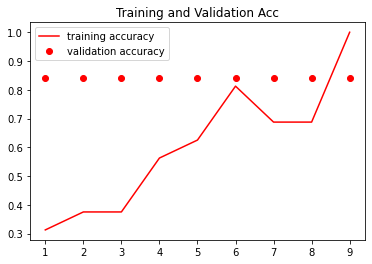
\includegraphics[width=1\textwidth,height=5cm,keepaspectratio]{Images/ThirdCNNBaselineTrainAndValAccBeforePreprocessing.png}\\
    \caption{Figure of Train and Validation Accuracy of Third CNN Baseline Model(Before Image Standardisation)}
    \label{fig:Third CNN Baseline Train and Validation Accuracy(Before Image Standardisation)}
\end{figure}
 \begin{figure}[H]
    \centering
    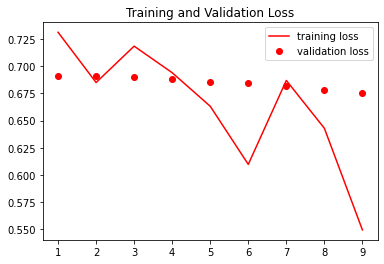
\includegraphics[width=1\textwidth,height=5cm,keepaspectratio]{Images/ThirdCNNBaselineTrainAndValLossBeforePreprocessing.png}\\
    \caption{Figure of Train and Validation Loss of Third CNN Baseline Model(Before Image Standardisation)}
    \label{fig:Third CNN Baseline Train and Validation Loss(before Pre-processing}
\end{figure}
As shown in the table above \ref{tab:Third CNN baseline model results for COVID-19 Chest X-ray Dataset} the model has a high degree of loss and the accuracy isn't very good on either the training or the test set.  This is to be expected as resizing the images when inputting them into the model will distort the information present.  The use of GANs to generate the data in a standardised resolution may help to mitigate this issue but as shown in the baseline model the lack of a uniform resolution for the images has led to poor performance.
\section{GAN Baseline Design and Comparison}
\subsection{GANs for Radiography Dataset}
Due to a large imbalance between classes in the dataset I decided to explore the use of GANs to create synthetic data for both the COVID positive images which comprise 7,232 images in this dataset and the Pneumonia positive images which comprise 2,690 images.  The normal class(healthy patients) is very over-represented in the data as it is comprised of 20,384 images, due to this imbalance the CNNs trained from this dataset will be heavily biased towards identifying the normal patients.  For this reason I have chose to use a number of Generative Adversarial Architectures to synthetically augment the classes lacking in data to balance the dataset and increase the generalization and robustness of the CNN models.
\subsection{VAE(Variational Auto Encoder)}
\subsubsection{COVID-19 Class Augmentation}
\subsubsection{Pneumonia Class Augmentation}

\subsection{DCGAN(Deep Convolutional GAN Network)}
\subsubsection{COVID-19 Class Augmentation}
When designing the DCGAN I experimented with a number of architectures, some of these architectures led to the GAN only producing black squares which was a sign of mode collapse.  Mode collapse occurs when the discriminator gets stuck at a local minimum and the generator learns to only produce the same type of image over and over again to fool the discriminator. I found switching from an ADAM optimizer to RMSPROP and experimenting with the learning rate and momentum led to far better results.  The model produced some promising results but a few of the X-Rays didn't appear to be the best of quality.  The lack of data was a challenge when training the DCGAN model as I only had 7,232 images to train with including the masks.    The following architecture was used to create the generator and discriminator:
\begin{minted}[linenos,tabsize=2,breaklines]{JavaScript}
discriminator = keras.Sequential(
    [
        keras.Input(shape=(128, 128, 3)),
        layers.Conv2D(64, kernel_size=4, strides=2, padding="same"),
        layers.LeakyReLU(alpha=0.5),
        layers.Conv2D(128, kernel_size=4, strides=2, padding="same"),
        layers.LeakyReLU(alpha=0.5),
        layers.Conv2D(128, kernel_size=4, strides=2, padding="same"),
        layers.LeakyReLU(alpha=0.5),
        layers.Flatten(),
        layers.Dropout(0.2),
        layers.Dense(1, activation="sigmoid"),
    ],
    name="discriminator",
)
discriminator.summary()

# Create the generator.
generator = keras.Sequential(
    [
        keras.Input(shape=(latent_dim,)),
        layers.Dense(8 * 8 * 128),
        layers.Reshape((8, 8, 128)),
        layers.Conv2DTranspose(256, kernel_size=4, strides=2, padding="same"),
        layers.LeakyReLU(alpha=0.2),
        layers.Conv2DTranspose(512, kernel_size=4, strides=2, padding="same"),
        layers.LeakyReLU(alpha=0.2),
        layers.Conv2DTranspose(1024, kernel_size=4, strides=2, padding="same"),
        layers.LeakyReLU(alpha=0.2),
        layers.Conv2DTranspose(64, kernel_size=4, strides=2, padding="same"),
        layers.LeakyReLU(alpha=0.2),
        layers.Conv2D(3, kernel_size=5, padding="same", activation="sigmoid"),
    ],
    name="generator",
)
generator.summary()
\end{minted}
The design of this GAN was based off of a Keras tutorial and the code was refactored for the purposes of this project\cite{DCGANKerasTutorial}.  The following hyper parameters were used when training the DCGAN model to generate synthetic COVID-19 X-Ray images: 
\begin{table}[H]
    \centering
    \resizebox{\textwidth}{!}{
    \begin{tabular}{|c|c|c|c|c|c|c|c|c|}
    \hline
         Generator Optimizer
         & Discriminator Optimizer 
         & Generator Learning Rate
         & Discriminator Learning Rate
         & Generator Momentum
         & Discriminator Momentum
         & Steps per Epoch
         & Batch Size
         & Number of Epochs\\
         \hline
         RMSPROP & RMSPROP & $1 \times 10 ^ -4$ & $1 \times 10 ^ -4$ & $1 \times 10 ^ -2$ & $1 \times 10 ^ -2$ & 1 & 16 & 452\\
         \hline
    \end{tabular}
    }
    \caption{DCGAN for Producing Synthetic Data From Radiography Dataset }
    \label{tab:DCGAN for Producing Synthetic Data From Radiography Dataset}
\end{table}
With this model architecture I was able to achieve a final score of 0.6094\% for the discriminator and 0.8001\% for the generator.
% include example images here produced from this GAN
\subsubsection{Pneumonia Class Augmentation}
The training of the DCGAN for the Pneumonia class took a lot of trial and error when training the GAN, as there is far less training data available for this class in comparison to the COVID class.  The Pneumonia class contains 2690 images of both the X-Rays and their masks, the COVID class contained 7,232 images for comparison which amounts to 4,542 more images.  It is clear to see the imbalance in this dataset given the difference between the various classes of which it is comprised.   During the training of this DCGAN I experimented with multiple hyper-parameters and trained many different GAN models.
\subsection{GANs for Chest X-Ray Dataset}
\subsection{GANs for X-Ray Dataset COVID-19}

\section{Improving CNN Models}
\section{Improving GAN Models}
\section{GANs in Conjunction}
\section{Conclusion}



\chapter{Results of Research and Conclusions}
\section{Evaluation of CNN Models}
\subsection{Radiography CNN Models}
\subsection{Chest X-Ray CNN Models}
\subsection{X-Ray Dataset Covid 19 CNN Models}
\section{Evaluation of GAN Models}
\subsection{Radiography GAN Models}
\subsubsection{Radiography DCGAN for COVID-19 Augmentation}
The radiography DCGAN for synthetically generated COVID-19 samples had mixed results.  Some of the images generated by the DCGAN came out looking very similar to the masks of patients lungs which were in the database.  I have included a side by side comparison in figure \ref{fig:Real COVID-19 Radiography Mask Example} and \ref{fig:Synthetically Generated COVID-19 Radiography Mask Example DCGAN} below
 \begin{figure}[H]
    \centering
    \begin{subfigure}{.5\textwidth}
    \centering
      
\includegraphics[width=.4\linewidth,keepaspectratio]{Images/Radiography_Real_Mask_COVID19_Example.png}
      \caption{Real COVID-19 Radiography Mask Example}
      \label{fig:Real COVID-19 Radiography Mask Example}
    \end{subfigure}%
    \begin{subfigure}{.5\textwidth}
    \centering
      
\includegraphics[width=.4\linewidth,keepaspectratio]{Images/Radiography_GAN_Mask_COVID19_Example.png}
      \caption{Generated COVID-19 Radiography Mask Example DCGAN}
      \label{fig:Synthetically Generated COVID-19 Radiography Mask Example DCGAN}
    \end{subfigure}%
\end{figure}
As is shown in the above images the synthetically generated COVID-19 mask looks relatively similar to the example taken from the dataset.  However not every single generated image came out as well as those that I have shown for demonstration purposes.  From reviewing the generated images it appears that a number of images bear no resemblance(or very little resemblance) to images within the data set.   
\\
From training a number of models there appears to be a need for pruning out bad images generated by the GAN and determining which images resemble X-Rays and Masks and which are "garbage" images which don't resemble data in our dataset.  This will require a lot of manual effort in determing which generated images are worth including in the augmented dataset and which are worth throwing away.
\subsection{Chest X-Ray GAN Models}
\subsection{X-Ray Dataset Covid 19 GAN Models}
\section{Possible Improvements}
\subsection{Larger Models}
\subsection{More Data Collection for GAN / CNN Training}
\subsection{More Computational Resources}
\section{Conclusion}
\chapter{Future Work and Research}
\section{Limitations}
\subsection{Computational Resources Offered by Google Colab Pro}
Due to limitations with Google Colab Pro I wasn't able to surpass certain limits when training the Convolutional Neural Networks and Generative Adversarial Networks.  This means that the number of units per layer of each model could not surpass a certain limit as the runtime would run out of memory and processing power.  The model's performance may be improved in future experiments when more computational power is available.   
\\
Due to this limitation I was only able to train models with approximately 10 to 20 million unit parameters depending on a number of factors such as the hyper parameters of the model.  The lack of computational resources also affected the GANs as I was not able to use high resolutions for the images and settled for a smaller resolution when training them on the images, as higher resolutions are more computationally expensive.
\subsection{Run time Limits in Google Colab Pro}
Due to run time limits I was also frequently met with disconnects when training larger models, this meant that during the process of training the model the run time would disconnect and I would be forced to run the model again.  This is due to Google conserving computational resources and limiting the amount of time a model can train while being idle.  I was able to mitigate this somewhat by following advice from a stack overflow post and including the following code:
\begin{minted}[linenos,tabsize=2,breaklines]{JavaScript}
import IPython
js_code = '''
function ClickConnect(){
console.log("Working");
document.querySelector("colab-toolbar-button#connect").click()
}
setInterval(ClickConnect,60000)
'''
IPython.display.Javascript(js_code)
\end{minted}
The above code was used to click the connect button after a certain amount of time to ensure the runtime was not disconnected.  There was however an limit to the amount of time this code could be run without the notebook disconnecting which was estimated to be approximately 24 hours.
\subsection{Lack of Data}
During the course of this study I was met with a desire for more data to use to train the GANs and CNNs, I found that the data in the classes which needed augmenting was not nearly enough to train a Generative Adversarial Model to produce perfect X-Rays nor to train a CNN to increase it's generalization ability.  This greatly hindered progress when training the GANs as mode collapse frequently occurred and tended to produce black square images which looked just enough like X-Rays to fool the discriminator.  If more data were available it may have mitigated a lot of the problems which occurred during the training of the GANs and possibly would have led to more realistic X-Rays being produced and a more various selection of X-Rays.  
\subsection{Time}
Time was a major limitation during the writing of this thesis as Convolutional Neural Networks and Generative Adversarial Models can take a very long time to train and develop.  Due to the time-consuming trial and error effort of adjusting the hyper parameters of models and rerunning the models to compare results of previous implementations I was spending a lot of my time waiting for models to train so that I could analyze the results.  This became especially cumbersome as mode collapse occurred many times when training the GANs.  The issue of time was also exacerbated by the computational limits of Google Colab which only allows a certain amount of memory and computational power to be allocated to the user. 
\section{Future Research}
\subsection{Suggestions for Future Research}
\subsubsection{Advancements in The Field of Artificial Intelligence}
At the time this thesis was written, \today, there has been much research and many advancements taking place in regards to Generative Adversarial Networks, Convolutional Neural Networks, synthetic data generation, and in the overall field of Artificial Intelligence.  I advise researchers who wish to expand on this problem domain and this research to research new methodologies and advances in this field as technology moves at such a rapid pace and undoubtedly the implementation of the networks contained within this thesis will become archaic and under perform in comparison to the latest and greatest implementations of such networks.
\\
The use of synthetic data appears to contain great promise for making data more ubiquitous and to encourage many people to enter the field of Machine Learning and Artificial Intelligence due to the abundance of data throughout various fields.  Not only could the generation of synthetic data encourage new people to enter the fields of Machine Learning and Artificial Intelligence, but it would also yield more robust models of CNNs and machine learning models in general which will perhaps be able to generalize better than our current models and assist experts in a variety of fields.
\subsubsection{Conducting Experiments with More Data}
With more data around COVID-19 becoming public it may be possible at a future date to conduct these experiments with more data.  More data would have greatly improved the training and performance of both the Convolutional Neural Networks and Generative Adversarial Networks.  Advancements in medical imaging technology may also have a positive effect upon future research as would the use of standardised and high quality datasets.  
\\
I would therefore advise those looking to expand upon this research to seek out more datasets which will hopefully be more readily available in the future. 
\section{Conclusion of Work}
\subsection{Issues Faced and How They Should be Mitigated in Future Research}
\subsubsection{Slow Training of Models Due to Lack of Computational Resources}
\subsection{Summary of Results}
\subsubsection{Analysis of Results and Their Significance}
\subsection{Final Words}
\printbibliography
\end{document}